% !TEX program = lualatex
% latexmk -lualatex docs/ueshm.tex
\documentclass[aspectratio=169,11pt]{beamer}

\usefonttheme{professionalfonts}
\usepackage{fontspec}
\defaultfontfeatures{Ligatures=TeX,Renderer=HarfBuzz}
\setsansfont{Avenir Next}[
  UprightFont={Avenir Next},
  BoldFont={Avenir Next Demi Bold},
  ItalicFont={Avenir Next Italic},
  BoldItalicFont={Avenir Next Demi Bold Italic},
]
\setmainfont{Avenir Next}[
  UprightFont={Avenir Next},
  BoldFont={Avenir Next Demi Bold},
  ItalicFont={Avenir Next Italic},
  BoldItalicFont={Avenir Next Demi Bold Italic},
]
\setmonofont{Menlo}[Scale=0.86]
\renewcommand{\familydefault}{\sfdefault}

\usepackage{microtype}
\usepackage{tikz}
\usetikzlibrary{arrows.meta,calc}

\definecolor{ink}{HTML}{1B2430}
\definecolor{muted}{HTML}{5C6B78}
\definecolor{accent}{HTML}{C4622D}
\definecolor{navy}{HTML}{17344F}
\definecolor{navyfill}{HTML}{E6EEF6}
\definecolor{eng}{HTML}{1A5C49}
\definecolor{engfill}{HTML}{E3F2EC}
\definecolor{hdrfill}{HTML}{E7EDF3}
\definecolor{cmdfill}{HTML}{D5E5F4}
\definecolor{rspfill}{HTML}{D4F0E4}
\definecolor{bulkfill}{HTML}{F8EFE3}
\definecolor{skipfill}{HTML}{E7E2DA}
\definecolor{cardline}{HTML}{D9D5CE}

\newcommand{\diagramfont}{\fontsize{12}{15}\selectfont}
\newcommand{\minorfont}{\fontsize{10}{13}\selectfont}
\newcommand{\microfont}{\fontsize{9}{11}\selectfont}

\tikzset{
  every node/.style={font=\diagramfont, text=ink, inner sep=2pt, align=center},
  every picture/.style={line cap=round, line join=round, x=1cm, y=1cm},
  stealth/.style={-{Stealth[length=2.15mm,width=1.7mm]}, line width=0.95pt},
  clock/.pic={
    \draw[line width=0.9pt] (0,0) circle[radius=0.28];
    \fill (0,0) circle[radius=0.042];
    \draw[line width=0.75pt] (0,0) -- (90:0.175);
    \draw[line width=0.75pt] (0,0) -- (30:0.12);
  },
}

% Schematic 16 MiB map. Fractions are not the real sizes.
% Leaves coordinates b0..b4 at the boundaries and hc, cc, rc, uc at the centers.
\newcommand{\MemoryMap}[2]{%
  \pgfmathsetmacro{\xa}{0.120*#1}%
  \pgfmathsetmacro{\xb}{0.362*#1}%
  \pgfmathsetmacro{\xc}{0.604*#1}%
  \begin{scope}
    \clip[rounded corners=3pt] (0,0) rectangle (#1,#2);
    \fill[hdrfill] (0,0) rectangle (\xa,#2);
    \fill[cmdfill] (\xa,0) rectangle (\xb,#2);
    \fill[rspfill] (\xb,0) rectangle (\xc,#2);
    \fill[bulkfill] (\xc,0) rectangle (#1,#2);
    \draw[white, line width=1.8pt] (\xa,0) -- (\xa,#2);
    \draw[white, line width=1.8pt] (\xb,0) -- (\xb,#2);
    \draw[white, line width=1.8pt] (\xc,0) -- (\xc,#2);
  \end{scope}
  \draw[ink!30, line width=0.8pt, rounded corners=3pt] (0,0) rectangle (#1,#2);
  \coordinate (b0) at (0,0);
  \coordinate (b1) at (\xa,0);
  \coordinate (b2) at (\xb,0);
  \coordinate (b3) at (\xc,0);
  \coordinate (b4) at (#1,0);
  \coordinate (hc) at ({0.5*\xa},{0.5*#2});
  \coordinate (cc) at ({0.5*\xa+0.5*\xb},{0.5*#2});
  \coordinate (rc) at ({0.5*\xb+0.5*\xc},{0.5*#2});
  \coordinate (uc) at ({0.5*\xc+0.5*#1},{0.5*#2});
}

\setbeamercolor{normal text}{fg=ink,bg=white}
\setbeamercolor{background canvas}{bg=white}
\setbeamercolor{frametitle}{fg=ink,bg=white}
\setbeamercolor{framesubtitle}{fg=muted}
\setbeamerfont{frametitle}{series=\bfseries,size*={17}{20}}
\setbeamerfont{itemize/enumerate body}{size*={11}{13.5}}
\setbeamerfont{itemize/enumerate item}{size*={11}{13.5}}
\setbeamercolor{itemize item}{fg=muted}
\setbeamertemplate{itemize item}{\scriptsize\textbullet}
\setbeamertemplate{navigation symbols}{}
\setbeamersize{text margin left=10mm, text margin right=10mm}

\setbeamertemplate{frametitle}{%
  \vspace*{1.8mm}%
  \begin{beamercolorbox}[wd=\paperwidth,leftskip=10mm,rightskip=10mm,sep=0pt]{frametitle}
    \usebeamerfont{frametitle}\insertframetitle\hfill
    {\microfont\color{muted}\insertframenumber\ /\ \inserttotalframenumber}\par
    \vspace{1.1mm}%
    {\color{accent}\rule{18mm}{1.15pt}}\par
  \end{beamercolorbox}%
  \vspace{1.4mm}%
}

\setbeamertemplate{footline}{}

\newcommand{\points}[1]{%
  \begingroup
  \setlength{\leftmargini}{1.05em}%
  \begin{itemize}\setlength\itemsep{0.9mm}\setlength\parsep{0pt}\setlength\topsep{0.4mm}%
    #1%
  \end{itemize}%
  \endgroup
  \vspace{1.6mm}%
}

\hypersetup{hidelinks,pdftitle={ueshm}}

\begin{document}

\begin{frame}
  \frametitle{Shared region}
  \points{%
    \item \texttt{uectl} creates the 16 MiB region and the editor process.
    \item \texttt{UEShmBridge} opens that name, passed as \texttt{-ShmName}.
    \item Both sides poll atomics. The region has no lock.%
  }

  \noindent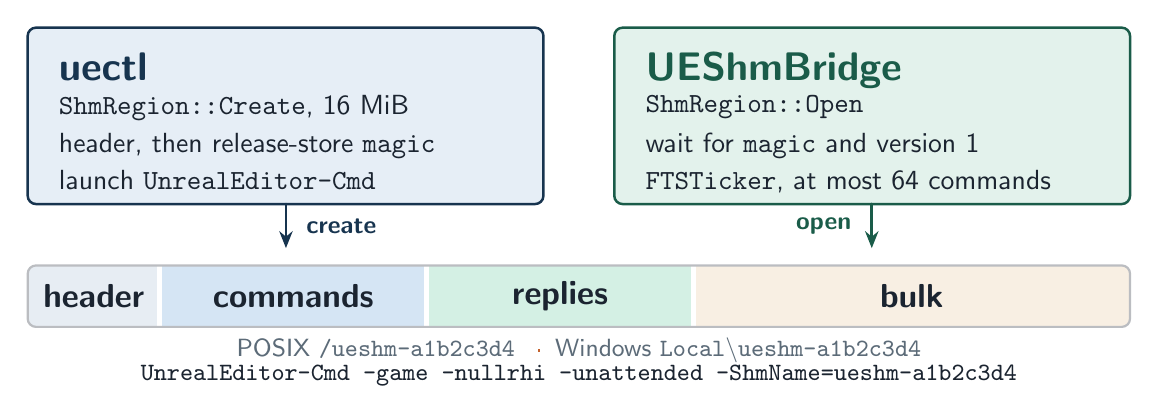
\begin{tikzpicture}
    \useasboundingbox (0,0) rectangle (14.00,4.52);
    \draw[navy, fill=navyfill, line width=0.9pt, rounded corners=3pt]
      (0,2.28) rectangle (6.55,4.52);
    \draw[eng, fill=engfill, line width=0.9pt, rounded corners=3pt]
      (7.45,2.28) rectangle (14.00,4.52);

    \node[anchor=north west, font=\fontsize{14}{17}\selectfont\bfseries, text=navy, align=left]
      at (0.32,4.28) {uectl};
    \node[anchor=north west, align=left, font=\minorfont] at (0.32,3.74)
      {\texttt{ShmRegion::Create}, 16 MiB};
    \node[anchor=north west, align=left, font=\minorfont] at (0.32,3.26)
      {header, then release-store \texttt{magic}};
    \node[anchor=north west, align=left, font=\minorfont] at (0.32,2.78)
      {launch \texttt{UnrealEditor-Cmd}};

    \node[anchor=north west, font=\fontsize{14}{17}\selectfont\bfseries, text=eng, align=left]
      at (7.77,4.28) {UEShmBridge};
    \node[anchor=north west, align=left, font=\minorfont] at (7.77,3.74)
      {\texttt{ShmRegion::Open}};
    \node[anchor=north west, align=left, font=\minorfont] at (7.77,3.26)
      {wait for \texttt{magic} and version 1};
    \node[anchor=north west, align=left, font=\minorfont] at (7.77,2.78)
      {\texttt{FTSTicker}, at most 64 commands};

    \draw[stealth, navy] (3.28,2.28) -- (3.28,1.72);
    \draw[stealth, eng] (10.72,2.28) -- (10.72,1.72);
    \node[font=\microfont\bfseries, text=navy, anchor=west, inner sep=1.5pt] at (3.48,2.00) {create};
    \node[font=\microfont\bfseries, text=eng, anchor=east, inner sep=1.5pt] at (10.52,2.00) {open};

    \begin{scope}[shift={(0,0.72)}]
      \MemoryMap{14.00}{0.78}
      \node[font=\diagramfont\bfseries] at (hc) {header};
      \node[font=\diagramfont\bfseries] at (cc) {commands};
      \node[font=\diagramfont\bfseries] at (rc) {replies};
      \node[font=\diagramfont\bfseries] at (uc) {bulk};
    \end{scope}

    \node[font=\microfont, text=muted] at (7.00,0.42)
      {POSIX \texttt{/ueshm-a1b2c3d4}
       \enspace{\color{accent}\textperiodcentered}\enspace
       Windows \texttt{Local\textbackslash ueshm-a1b2c3d4}};
    \node[font=\microfont] at (7.00,0.10)
      {\texttt{UnrealEditor-Cmd -game -nullrhi -unattended -ShmName=ueshm-a1b2c3d4}};
  \end{tikzpicture}
\end{frame}

\begin{frame}
  \frametitle{Region layout}
  \points{%
    \item Widths are schematic. Offsets are bytes. 16 MiB is 16777216.
    \item \texttt{magic} \texttt{0x48534555}, written last. version 1. state 0, 1, or 2.
    \item Heartbeats on each poll and tick. Acquire the counter before reading.%
  }

  \noindent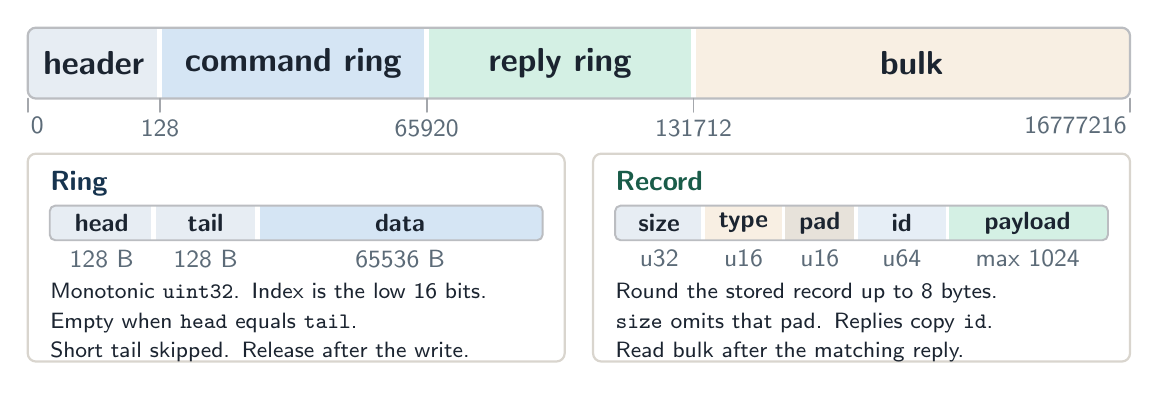
\begin{tikzpicture}
    \useasboundingbox (0,-0.08) rectangle (14.00,4.22);
    \begin{scope}[shift={(0,3.32)}]
      \MemoryMap{14.00}{0.90}
      \node[font=\diagramfont\bfseries] at (hc) {header};
      \node[font=\diagramfont\bfseries] at (cc) {command ring};
      \node[font=\diagramfont\bfseries] at (rc) {reply ring};
      \node[font=\diagramfont\bfseries] at (uc) {bulk};
    \end{scope}

    \draw[ink!40, line width=0.6pt] (b0) -- ([yshift=-1.7mm]b0);
    \draw[ink!40, line width=0.6pt] (b1) -- ([yshift=-1.7mm]b1);
    \draw[ink!40, line width=0.6pt] (b2) -- ([yshift=-1.7mm]b2);
    \draw[ink!40, line width=0.6pt] (b3) -- ([yshift=-1.7mm]b3);
    \draw[ink!40, line width=0.6pt] (b4) -- ([yshift=-1.7mm]b4);
    \node[font=\microfont, text=muted, anchor=north west, inner sep=1pt] at ([yshift=-2.0mm]b0) {0};
    \node[font=\microfont, text=muted, anchor=north] at ([yshift=-2.0mm]b1) {128};
    \node[font=\microfont, text=muted, anchor=north] at ([yshift=-2.0mm]b2) {65920};
    \node[font=\microfont, text=muted, anchor=north] at ([yshift=-2.0mm]b3) {131712};
    \node[font=\microfont, text=muted, anchor=north east, inner sep=1pt] at ([yshift=-2.0mm]b4) {16777216};

    \draw[cardline, line width=0.8pt, rounded corners=3pt, fill=white]
      (0,-0.02) rectangle (6.82,2.62);
    \node[anchor=north west, font=\minorfont\bfseries, text=navy, align=left, inner sep=0pt]
      at (0.28,2.40) {Ring};
    \begin{scope}[shift={(0.28,1.52)}]
      \def\ra{1.32}\def\rb{2.64}\def\rw{6.26}\def\rh{0.44}
      \begin{scope}
        \clip[rounded corners=2pt] (0,0) rectangle (\rw,\rh);
        \fill[hdrfill] (0,0) rectangle (\rb,\rh);
        \fill[cmdfill] (\rb,0) rectangle (\rw,\rh);
        \draw[white, line width=1.6pt] (\ra,0) -- (\ra,\rh);
        \draw[white, line width=1.6pt] (\rb,0) -- (\rb,\rh);
      \end{scope}
      \draw[ink!30, line width=0.7pt, rounded corners=2pt] (0,0) rectangle (\rw,\rh);
      \node[font=\microfont\bfseries] at (0.66,0.22) {head};
      \node[font=\microfont\bfseries] at (1.98,0.22) {tail};
      \node[font=\microfont\bfseries] at (4.45,0.22) {data};
      \node[font=\microfont, text=muted, anchor=north] at (0.66,-0.05) {128 B};
      \node[font=\microfont, text=muted, anchor=north] at (1.98,-0.05) {128 B};
      \node[font=\microfont, text=muted, anchor=north] at (4.45,-0.05) {65536 B};
    \end{scope}
    \node[anchor=north west, align=left, font=\fontsize{8.5}{10.6}\selectfont, text width=6.30cm, inner sep=0pt]
      at (0.28,0.98)
      {Monotonic \texttt{uint32}. Index is the low 16 bits.\\
       Empty when \texttt{head} equals \texttt{tail}.\\
       Short tail skipped. Release after the write.};

    \draw[cardline, line width=0.8pt, rounded corners=3pt, fill=white]
      (7.18,-0.02) rectangle (14.00,2.62);
    \node[anchor=north west, font=\minorfont\bfseries, text=eng, align=left, inner sep=0pt]
      at (7.46,2.40) {Record};
    \begin{scope}[shift={(7.46,1.52)}]
      \def\rh{0.44}
      \begin{scope}
        \clip[rounded corners=2pt] (0,0) rectangle (6.26,\rh);
        \fill[hdrfill] (0,0) rectangle (1.12,\rh);
        \fill[bulkfill] (1.12,0) rectangle (2.14,\rh);
        \fill[skipfill] (2.14,0) rectangle (3.06,\rh);
        \fill[navyfill] (3.06,0) rectangle (4.22,\rh);
        \fill[rspfill] (4.22,0) rectangle (6.26,\rh);
        \draw[white, line width=1.3pt] (1.12,0) -- (1.12,\rh);
        \draw[white, line width=1.3pt] (2.14,0) -- (2.14,\rh);
        \draw[white, line width=1.3pt] (3.06,0) -- (3.06,\rh);
        \draw[white, line width=1.3pt] (4.22,0) -- (4.22,\rh);
      \end{scope}
      \draw[ink!30, line width=0.7pt, rounded corners=2pt] (0,0) rectangle (6.26,\rh);
      \node[font=\microfont\bfseries] at (0.56,0.22) {size};
      \node[font=\microfont\bfseries] at (1.63,0.22) {type};
      \node[font=\microfont\bfseries] at (2.60,0.22) {pad};
      \node[font=\microfont\bfseries] at (3.64,0.22) {id};
      \node[font=\microfont\bfseries] at (5.24,0.22) {payload};
      \node[font=\microfont, text=muted, anchor=north] at (0.56,-0.05) {u32};
      \node[font=\microfont, text=muted, anchor=north] at (1.63,-0.05) {u16};
      \node[font=\microfont, text=muted, anchor=north] at (2.60,-0.05) {u16};
      \node[font=\microfont, text=muted, anchor=north] at (3.64,-0.05) {u64};
      \node[font=\microfont, text=muted, anchor=north] at (5.24,-0.05) {max 1024};
    \end{scope}
    \node[anchor=north west, align=left, font=\fontsize{8.5}{10.6}\selectfont, text width=6.30cm, inner sep=0pt]
      at (7.46,0.98)
      {Round the stored record up to 8 bytes.\\
       \texttt{size} omits that pad. Replies copy \texttt{id}.\\
       Read bulk after the matching reply.};
  \end{tikzpicture}
\end{frame}

\begin{frame}
  \frametitle{PING round trip}
  \points{%
    \item Starts after \texttt{state} is 1 (\texttt{ue\_ready}).
    \item \texttt{PING} is type 1. \texttt{PONG} is type 101. \texttt{id} and the nonce are copied.
    \item \texttt{uectl} sleeps 10 ms between polls of the reply ring.%
  }

  \noindent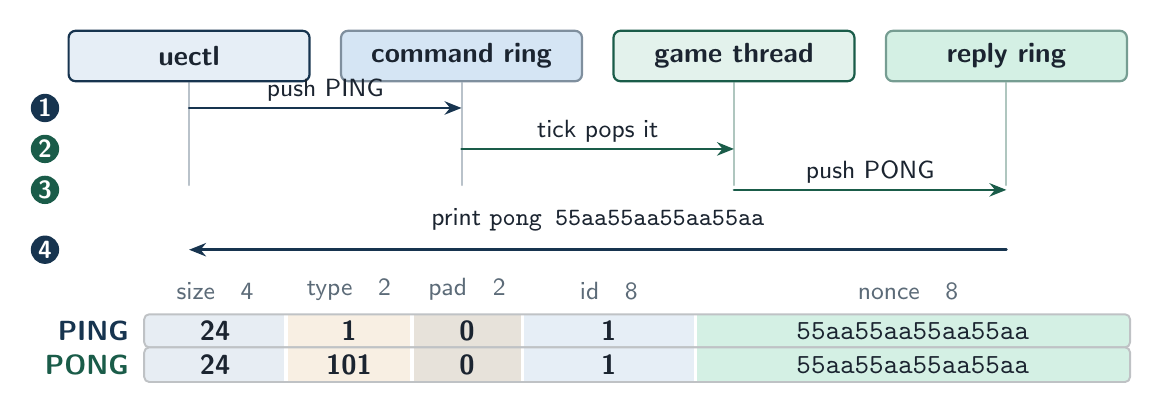
\begin{tikzpicture}
    \useasboundingbox (0,0) rectangle (14.00,4.52);
    \coordinate (a0) at (2.05,4.16);
    \coordinate (a1) at (5.51,4.16);
    \coordinate (a2) at (8.97,4.16);
    \coordinate (a3) at (12.43,4.16);

    \draw[navy!30, line width=0.7pt] (2.05,3.82) -- (2.05,2.52);
    \draw[navy!30, line width=0.7pt] (5.51,3.82) -- (5.51,2.52);
    \draw[eng!35, line width=0.7pt] (8.97,3.82) -- (8.97,2.52);
    \draw[eng!35, line width=0.7pt] (12.43,3.82) -- (12.43,2.52);

    \node[draw=navy, fill=navyfill, line width=0.8pt, rounded corners=2.5pt,
          minimum width=3.06cm, minimum height=0.64cm, font=\minorfont\bfseries] at (a0) {uectl};
    \node[draw=navy!55, fill=cmdfill, line width=0.8pt, rounded corners=2.5pt,
          minimum width=3.06cm, minimum height=0.64cm, font=\minorfont\bfseries] at (a1) {command ring};
    \node[draw=eng, fill=engfill, line width=0.8pt, rounded corners=2.5pt,
          minimum width=3.06cm, minimum height=0.64cm, font=\minorfont\bfseries] at (a2) {game thread};
    \node[draw=eng!60, fill=rspfill, line width=0.8pt, rounded corners=2.5pt,
          minimum width=3.06cm, minimum height=0.64cm, font=\minorfont\bfseries] at (a3) {reply ring};

    \draw[stealth, navy] (2.05,3.50) -- (5.51,3.50);
    \draw[stealth, eng] (5.51,2.98) -- (8.97,2.98);
    \draw[stealth, eng] (8.97,2.46) -- (12.43,2.46);
    \draw[stealth, navy] (12.43,1.70) -- (2.05,1.70);

    \node[font=\microfont, inner sep=1pt] at (3.78,3.72) {push PING};
    \node[font=\microfont, inner sep=1pt] at (7.24,3.20) {tick pops it};
    \node[font=\microfont, inner sep=1pt] at (10.70,2.68) {push PONG};
    \node[font=\microfont, inner sep=1pt] at (7.24,2.08)
      {print \texttt{pong 55aa55aa55aa55aa}};

    \foreach \y/\n/\col in {3.50/1/navy, 2.98/2/eng, 2.46/3/eng, 1.70/4/navy} {
      \fill[\col] (0.22,\y) circle[radius=0.18];
      \node[font=\microfont\bfseries, text=white] at (0.22,\y) {\n};
    }

    \begin{scope}[shift={(1.48,0)}]
      \node[font=\microfont, text=muted, anchor=south, inner sep=1pt] at (0.90,1.02) {size\quad 4};
      \node[font=\microfont, text=muted, anchor=south, inner sep=1pt] at (2.60,1.02) {type\quad 2};
      \node[font=\microfont, text=muted, anchor=south, inner sep=1pt] at (4.10,1.02) {pad\quad 2};
      \node[font=\microfont, text=muted, anchor=south, inner sep=1pt] at (5.90,1.02) {id\quad 8};
      \node[font=\microfont, text=muted, anchor=south, inner sep=1pt] at (9.70,1.02) {nonce\quad 8};
      \begin{scope}[shift={(0,0.46)}]
        \begin{scope}
          \clip[rounded corners=1.8pt] (0,0) rectangle (12.52,0.42);
          \fill[hdrfill] (0,0) rectangle (1.80,0.42);
          \fill[bulkfill] (1.80,0) rectangle (3.40,0.42);
          \fill[skipfill] (3.40,0) rectangle (4.80,0.42);
          \fill[navyfill] (4.80,0) rectangle (7.00,0.42);
          \fill[rspfill] (7.00,0) rectangle (12.52,0.42);
          \draw[white, line width=1.2pt] (1.80,0) -- (1.80,0.42);
          \draw[white, line width=1.2pt] (3.40,0) -- (3.40,0.42);
          \draw[white, line width=1.2pt] (4.80,0) -- (4.80,0.42);
          \draw[white, line width=1.2pt] (7.00,0) -- (7.00,0.42);
        \end{scope}
        \draw[ink!28, line width=0.7pt, rounded corners=1.8pt] (0,0) rectangle (12.52,0.42);
        \node[font=\minorfont\bfseries] at (0.90,0.21) {24};
        \node[font=\minorfont\bfseries] at (2.60,0.21) {1};
        \node[font=\minorfont\bfseries] at (4.10,0.21) {0};
        \node[font=\minorfont\bfseries] at (5.90,0.21) {1};
        \node[font=\minorfont] at (9.76,0.21) {\texttt{55aa55aa55aa55aa}};
      \end{scope}
      \begin{scope}[shift={(0,0.02)}]
        \begin{scope}
          \clip[rounded corners=1.8pt] (0,0) rectangle (12.52,0.44);
          \fill[hdrfill] (0,0) rectangle (1.80,0.44);
          \fill[bulkfill] (1.80,0) rectangle (3.40,0.44);
          \fill[skipfill] (3.40,0) rectangle (4.80,0.44);
          \fill[navyfill] (4.80,0) rectangle (7.00,0.44);
          \fill[rspfill] (7.00,0) rectangle (12.52,0.44);
          \draw[white, line width=1.2pt] (1.80,0) -- (1.80,0.44);
          \draw[white, line width=1.2pt] (3.40,0) -- (3.40,0.44);
          \draw[white, line width=1.2pt] (4.80,0) -- (4.80,0.44);
          \draw[white, line width=1.2pt] (7.00,0) -- (7.00,0.44);
        \end{scope}
        \draw[ink!28, line width=0.7pt, rounded corners=1.8pt] (0,0) rectangle (12.52,0.44);
        \node[font=\minorfont\bfseries] at (0.90,0.22) {24};
        \node[font=\minorfont\bfseries] at (2.60,0.22) {101};
        \node[font=\minorfont\bfseries] at (4.10,0.22) {0};
        \node[font=\minorfont\bfseries] at (5.90,0.22) {1};
        \node[font=\minorfont] at (9.76,0.22) {\texttt{55aa55aa55aa55aa}};
      \end{scope}
    \end{scope}
    \node[font=\minorfont\bfseries, text=navy, anchor=east] at (1.36,0.67) {PING};
    \node[font=\minorfont\bfseries, text=eng, anchor=east] at (1.36,0.24) {PONG};
  \end{tikzpicture}
\end{frame}

\begin{frame}
  \frametitle{Tool-driven timestep}
  \points{%
    \item Not implemented. The command ring and the reply ring stay as they are.
    \item Current: the engine advances time, then \texttt{FTSTicker} drains commands.
    \item Proposed: the frame waits until \texttt{uectl} sends a delta.%
  }

  \noindent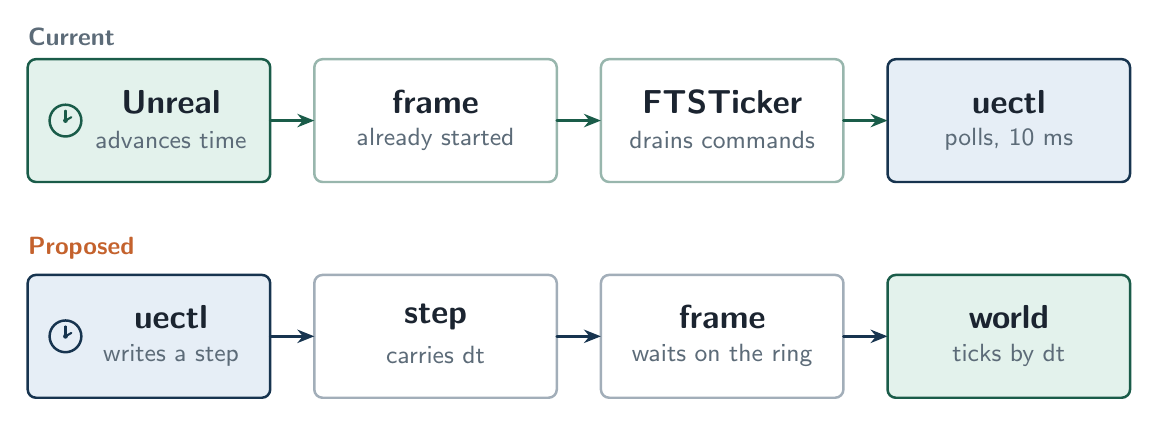
\begin{tikzpicture}
    \useasboundingbox (0,0) rectangle (14.00,4.88);
    \node[anchor=north west, font=\microfont\bfseries, text=muted, inner sep=0pt] at (0,4.88) {Current};
    \node[anchor=north west, font=\microfont\bfseries, text=accent, inner sep=0pt] at (0,2.22) {Proposed};

    \foreach \i/\name/\sub/\fillc/\drawc in {
      0/Unreal/{advances time}/engfill/eng,
      1/frame/{already started}/white/eng!45,
      2/FTSTicker/{drains commands}/white/eng!45,
      3/uectl/{polls, 10 ms}/navyfill/navy} {
      \pgfmathsetmacro{\x}{\i*3.64}
      \draw[\drawc, fill=\fillc, line width=0.9pt, rounded corners=3pt]
        (\x,2.92) rectangle ({\x+3.08},4.48);
      \ifnum\i=0
        \pic[draw=eng, fill=eng, scale=0.72] at ({\x+0.48},3.70) {clock};
        \node[font=\fontsize{13}{16}\selectfont\bfseries] at ({\x+1.82},3.94) {\name};
        \node[font=\microfont, text=muted] at ({\x+1.82},3.46) {\sub};
      \else
        \node[font=\fontsize{13}{16}\selectfont\bfseries] at ({\x+1.54},3.94) {\name};
        \node[font=\microfont, text=muted] at ({\x+1.54},3.46) {\sub};
      \fi
    }
    \draw[stealth, eng] (3.08,3.70) -- (3.64,3.70);
    \draw[stealth, eng] (6.72,3.70) -- (7.28,3.70);
    \draw[stealth, eng] (10.36,3.70) -- (10.92,3.70);

    \foreach \i/\name/\sub/\fillc/\drawc in {
      0/uectl/{writes a step}/navyfill/navy,
      1/step/{carries dt}/white/navy!40,
      2/frame/{waits on the ring}/white/navy!40,
      3/world/{ticks by dt}/engfill/eng} {
      \pgfmathsetmacro{\x}{\i*3.64}
      \draw[\drawc, fill=\fillc, line width=0.9pt, rounded corners=3pt]
        (\x,0.18) rectangle ({\x+3.08},1.74);
      \ifnum\i=0
        \pic[draw=navy, fill=navy, scale=0.72] at ({\x+0.48},0.96) {clock};
        \node[font=\fontsize{13}{16}\selectfont\bfseries] at ({\x+1.82},1.20) {\name};
        \node[font=\microfont, text=muted] at ({\x+1.82},0.72) {\sub};
      \else
        \node[font=\fontsize{13}{16}\selectfont\bfseries] at ({\x+1.54},1.20) {\name};
        \node[font=\microfont, text=muted] at ({\x+1.54},0.72) {\sub};
      \fi
    }
    \draw[stealth, navy] (3.08,0.96) -- (3.64,0.96);
    \draw[stealth, navy] (6.72,0.96) -- (7.28,0.96);
    \draw[stealth, navy] (10.36,0.96) -- (10.92,0.96);
  \end{tikzpicture}
\end{frame}

\end{document}
